\documentclass[conference]{IEEEtran}
\IEEEoverridecommandlockouts
% The preceding line is only needed to identify funding in the first footnote. If that is unneeded, please comment it out.
\usepackage{cite}
\usepackage{amsmath,amssymb,amsfonts}
\usepackage{algorithmic}
\usepackage{graphicx}
\usepackage{textcomp}
\usepackage{xcolor}
% mine own
% \usepackage{caption}
\usepackage{tabularx}
\def\BibTeX{{\rm B\kern-.05em{\sc i\kern-.025em b}\kern-.08em
    T\kern-.1667em\lower.7ex\hbox{E}\kern-.125emX}}
\begin{document}

\title{Collaborative Networks in Machine Learning Hardware\\
\thanks{University of Texas at Austin}
}

\author{\IEEEauthorblockN{1\textsuperscript{st} Given Name Surname}
\IEEEauthorblockA{\textit{dept. name of organization (of Aff.)} \\
\textit{name of organization (of Aff.)}\\
City, Country \\
email address or ORCID}
\and
\IEEEauthorblockN{2\textsuperscript{nd} Given Name Surname}
\IEEEauthorblockA{\textit{dept. name of organization (of Aff.)} \\
\textit{name of organization (of Aff.)}\\
City, Country \\
email address or ORCID}
\and
\IEEEauthorblockN{3\textsuperscript{rd} Given Name Surname}
\IEEEauthorblockA{\textit{dept. name of organization (of Aff.)} \\
\textit{name of organization (of Aff.)}\\
City, Country \\
email address or ORCID}
\and
\IEEEauthorblockN{4\textsuperscript{th} Given Name Surname}
\IEEEauthorblockA{\textit{dept. name of organization (of Aff.)} \\
\textit{name of organization (of Aff.)}\\
City, Country \\
email address or ORCID}
\and
\IEEEauthorblockN{5\textsuperscript{th} Given Name Surname}
\IEEEauthorblockA{\textit{dept. name of organization (of Aff.)} \\
\textit{name of organization (of Aff.)}\\
City, Country \\
email address or ORCID}
\and
\IEEEauthorblockN{5\textsuperscript{th} Given Name Surname}
\IEEEauthorblockA{\textit{dept. name of organization (of Aff.)} \\
\textit{name of organization (of Aff.)}\\
City, Country \\
email address or ORCID}
}

\maketitle

\begin{abstract}
Citation networks are graphical networks composed of publications as nodes and citations as edges. 
They offer a unique look into scientific collaboration and the flow of knowledge within academia. 
In this paper, we examine the history of machine learning hardware papers through the lens of citation 
networks and construct GNN models for node classification and link prediction for our custom machine 
learning hardware dataset as well as existing datasets in software engineering and machine learning. 
We utilize existing citation graphs as well as curate our own dataset from the Web of Science database 
to show that node classification and link prediction are effective on a new network of machine learning 
hardware papers.
\end{abstract}

% \begin{IEEEkeywords}
% component, formatting, style, styling, insert
% \end{IEEEkeywords}

\section{Introduction and Motivation}
Inspired by the recent advent of graphical neural networks (GNNs), this project explores their potential to classify academic networks. 
Given any individual publication or author, GNNs could predict their relation to the remainder of the network, 
useful for understanding the relationships between academic fields, authors, institutions, and more. This opens the door to 
opportunities for classifying papers in fields with minimal representation in existing citation networks or predicting links 
between papers, potentially applicable to discovering inspiring papers related to an author's past work, 
among other capabilities. \par

In particular, machine learning hardware is a new field that has skyrocketed from the recent popularity of machine learning. 
Due to the compute-intensive nature of this field, plenty of research exists in the hardware infrastructure to support these 
computing loads. We utilize GNNs for node classification and link prediction to explore existing datasets and comment on the 
new corpus of machine learning hardware papers. The main challenges are processing data for useful representations of the network 
and data interpretation on the created GNNs to comment on the field of machine learning hardware. \par

\section{Previous Work}
There have been many previous explorations of citation networks using the datasets Cora, Citeseer, and PubMed Diabetes. 
In these citation networks, in particular, node classification and link prediction have been heavily explored. 
In Optimization of Graph Neural Networks with Natural Gradient Descent, Izadi et al improve on traditional optimization 
algorithms such as ADAM and stochastic gradient descent (SGD), producing a superior accuracy (90.16±0.59\%) 
by utilizing a proposed method inspired by natural gradient descent. This paper achieved the highest accuracy across 
71 different papers done on node classification of the Cora dataset \cite{CoraAccuracy}.  \par

Those that explored link prediction in the Cora and Citeseer datasets have achieved great results as well. 
In ‘NESS: Node Embeddings from Static SubGraphs,’ Ucar proposed splitting up the graph into multiple subgraphs 
that do not have overlapping edges in between subgraphs, using each graph to train and obtain node representations, 
then aggregating the results to obtain predictions. Using this, he was able to obtain state-of-the-art accuracy results, 
achieving 98.94±0.1\% on Citeseer and 96.81±0.6\% on Cora. \cite{Ucar}
These past studies show the efficacy of GNNs on academic publications for node classification and link prediction, and, 
since these accuracies were certainly impressive, we hope to use these networks as a baseline to examine the key features 
of different datasets and extract information to create a similar dataset about the subject of machine learning hardware.  \par

\section{Approach}

Two preconstructed datasets, Cora and CiteSeer, are large datasets of scientific machine learning papers. 
Each dataset contains papers from before 2008, with citations to other papers in the database as well as the 
vocabulary used. The nodes of the graph are the papers themselves, with topics and vocabulary as individual features, 
while the directed links are citations to other papers. Cora classifies each publication into one of seven categories: 
Theory, Reinforcement Learning, Genetic Algorithms, Neural Networks, Probabilistic Methods, Case Based, and Rule Learning. 
On the other hand, Citeseer classifies each publication into one of six categories: Agents, Artificial Intelligence, Database, 
Human Computer Interaction, Machine Learning, and Information Retrieval. \par

Meanwhile, PubMed is a database of diabetes publications that is classified into one of three classes \cite{Pubmed}. As such, this 
dataset is similar to both Cora and CiteSeer, though it further explores the efficacy of GNNs on datasets outside of 
machine learning. This performance of this dataset can further validate parameters potentially affecting accuracies, 
such as edge count, classes, or path length,  in addition to explaining differences in different fields of publications. \par

Web of Science (WoS) is an online database of publication citations and information \cite{WoS}. 
This online database created by Clarivate can be queried by genre and shows identifying information such as titles, 
references, and specific citations. As such, we can utilize the WoS dataset to address the goal of exploring additional 
datasets in machine learning hardware. Specifically, by downloading papers by (exclusive) topic, 
we can create a dataset representative of the field of machine learning and compare the performance of our dataset 
against GNNs alongside other common datasets to analyze its efficacy on these models and its viability as a dataset 
in an academic setting. Using this popular database, we query their dataset of publications for four categories: 
Machine Learning on the Edge, Neuromorphic Computing, Spiking Neural Networks, and Machine Learning Accelerator. 
In using the Web of Science database, we assume that the papers are representative of their assigned class and 
distinct from related classes. In this regard, the dataset that we curate is unique from other citation networks 
in that it will hold distinct characteristics and be of machine learning hardware, providing insight into the 
structure and nature of the machine learning hardware citation network. \par

Beginning with the provided models like Deep Graph Library, we take inspiration from existing methods, 
such as preprocessing methods discussed by the Semantic Scholar Academic Graph \cite{Wade}. By constructing our 
datasets of publications, we will examine model characteristics of varying types of publication networks. 
We also explored other datasets to improve the diversity of our datasets. The  Microsoft Open Academic Graph \cite{Sinha}, 
a large academic graph dataset, shows a promising example of dataset scale, though it has differences in 
features, scaling, and overlapping that can interfere with providing information about any one academic field. 
Here, the data set uses a variety of data types for the nodes, like publications, authors, and venues, with 
the links between each denoting a correlation. \par 

Following the specified approach to our project goals, the main tasks of our project are as follows. 
First, we will apply the necessary pre-processing techniques to each dataset for model compatibility. 
Then, we will create a GNN model using each dataset that accurately predicts paper topics and citations, 
commenting on the accuracy and effectiveness of GNNs in node classification or link prediction in academic 
contexts. For node classification, we will create a GNN model based on the vocabulary and neighbors as 
embeddings of each node, experimenting with different configurations to find the best model. Finally, 
we will take the results in terms of graph characteristics and model performance to analyze our dataset 
as an academic tool. In this regard, our technique is rather scalable, as these steps can be applied to 
academic datasets of nearly any field and in datasets beyond academic publications as well. However, 
this is also given the assumption that different academic fields follow similar citation networks to 
those listed, that these fields can be described by the vocabularies that they exhibit, and that 
these networks produce a graph that is compatible with neural network models. \par

\section{Experimental Setup and Results}

\subsection{Datasets}

Since the datasets Cora and Citeseer are included within some deep learning packages, 
we directly use those for constructing GNNs. Utilizing resources and configurations of 
included models within StellarGraph, Pytorch Geometric, and Keras, we can also construct 
predictive models for node classification and link prediction. \par

In creating our dataset, we query Web of Science for topics in machine learning 
hardware published between 1970 and 2022. For ease of use, we removed nodes without a 
DOI and duplicated values between categories so each node only belongs to one category. 
The collected data includes title, publishing year, abstract, and citations. \par

While Web of Science shows a close-to-linear growth of publications during this time, 
there has been an exponential growth of papers in machine learning hardware over the 
same period. We see a large spike in interest, following machine learning in general 
after OpenAI launched GPT. \par

With the text files generated, we constructed a NetworkX graph using DOI values to 
match paper citations. We also utilized the categories as labels, and the overall 
graph topography is in Figure A. This graph serves as our dataset once converted 
into StellarGraph or NetworkX Pytorch Geometric dataset instances as needed. \par 

In total, our graph had 4951 nodes, though only 2605 nodes have non-zero edges. 
Looking at the in-degrees of each node, we see evidence of a scale-free network, 
where few nodes are popularly cited, but many are not referenced often. This may 
also be due to the recentness of these publications, as future papers will likely 
add on to those numbers. The number of paper citations is also indicative of its 
impact, with larger in-degrees meaning more outreach and influence. \par 

Removing nodes without edges allows us to focus on the variety in edges and prevents 
the model from predicting 0 edges each time for high accuracy, the resulting is 
still disconnected, with an average degree of 5.0672, an average clustering coefficient 
of 0.1353, and a maximum diameter across all connected subgraphs of 16, 
with the average undirected path length being 4.6073 edges. \par 

However, from observation, we notice that our graph is much smaller and less connected 
than the given datasets. As in Figure 1 below, there are lots of unconnected nodes. 
And, after removing non-zero edges, there are still plenty of nodes that have only 
one edge to another paper, likely due to their remaining citations not having an associated 
word vector. \par 

To combat this, we increase the size of the WoS database, querying additional nodes from the 
WoS database. Then, we take the largest connected component of the 
larger graph to increase the overall connectivity of the graph. \par

\begin{figure}[htbp]
    \centerline{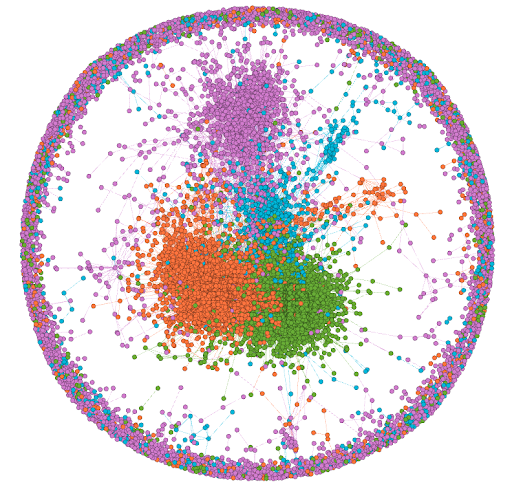
\includegraphics[scale=0.3] {wos_pic.png}}
    \caption{Large WoS network, Blue=ML Accelerators, Purple=Edge ML, Green=Neuromorphic Computing, Orange=Spiking Neural Network.}
    \label{fig}
\end{figure}

After applying these operations, the total number of nodes increases from 2,605 to 9,605 after removing 
unusable nodes. This graph also has 52,945 edges and 6,821 features, from applying the 
same methods of keyword extraction. When increasing the size of the dataset, we were also 
met with a class imbalance - there were far fewer papers in ML Accelerators in the WoS database, 
less than two thousand papers, while the other categories had over five thousand papers each. 
In this regard, we can infer that ML accelerators are less popular (or at least less explored) 
than other papers. However, since WoS is our only source of data, this could also result from 
a lack of these papers in the Web of Science database. Since class imbalances can also impact 
performance on ML models, this also acts as a limitation on the GNN models in use. \par

Recognizing that the number of features is nearly double that of any of the given datasets, 
this can also lead to excessive computation time and increased bias in the results from 
features that supply noise in the machine learning models. So, we then apply principal 
component analysis (PCA) to these features to select the features that best describe the 
classifications and links between each node. Here, we apply PCA with an explained variance 
of 80\% to provide a sufficient level of specificity without overfitting the data, 
reducing the number of features to 760. \par

Following this, we also update the characteristics of our graph, producing an average 
degree of 11.09, an average clustering coefficient of 0.158, and a diameter of 18. 
From the differences in these datasets, we see that the average degree of our dataset 
is much higher than the given datasets. However, the clustering coefficient and diameter 
of the dataset are comparable to those of other datasets. These metrics are compared to 
the other datasets in Table 1 below. \par 

From this table, we can see differences among the datasets explored in this paper, 
revealing the structural properties of these different graphs. Primarily, there are 
many more edges in the updated WoS compared to the other datasets, resulting in a much 
higher average degree for the updated dataset. However, the clustering coefficient for 
our dataset is still comparable to other datasets, implying that the field of machine 
learning hardware tends to have a significant number of citations, but a similar number 
of these papers forming a well-defined cluster. While Cora and CiteSeer are most similar 
to the WoS database in terms of content, both relating to machine learning, the graph 
characteristics of WoS are most similar to PubMed, with a higher degree and lower 
clustering coefficient. However, another limitation of utilizing WoS as our primary 
database is that it is unclear whether these characteristics arise as a quality of 
the database or as a characteristic of the field of ML hardware in general. \par

\begin{table}[htbp]
    \caption{Citation Network Characteristics}
    \begin{center}
        \begin{tabular}{|c|cccccc|}
        \hline
        \textbf{} & \textbf{\textit{Nodes}} & \textbf{\textit{Edges}} & \textbf{\textit{Features}} &
        \textbf{\textit{Degree}} & \textbf{\textit{CC$^{\mathrm{a}}$}} & \textbf{\textit{MD$^{\mathrm{b}}$}} \\
        \hline
        \textbf{\textit{Cora}} & 
        2708& 5429& 1433& 3.89807& 0.24067& 19 \\
        \textbf{\textit{CiteSeer}} & 
        3312& 4660& 3704& 2.81400& 0.14255& 28 \\
        \textbf{\textit{Pubmed}} & 
        19717& 44348& 500& 4.49632& 0.06017& 18 \\
        \textbf{\textit{Small WoS}} & 
        2605& 6600& 4134& 5.06717& 0.13529& 16 \\
        \textbf{\textit{Large WoS}} & 
        2605& 6600& 4134& 5.06717& 0.13529& 16 \\
        \hline
        \end{tabular}
        \label{tab1}
        {$^{\mathrm{a}}$Clustering Coefficient.}
        {$^{\mathrm{b}}$Maximum Diameter.}
    \end{center}
\end{table}

To see the distribution of the demographic of the papers in terms of age, 
we look at the number of papers in our updated WoS database, as in Figure 2 
below. From this graph, we see that papers have been released more frequently 
in recent years. This implies that machine learning hardware is a rising field, 
which follows given the recent popularity of machine learning as a field in general. \par

\begin{figure}[htbp]
    \centerline{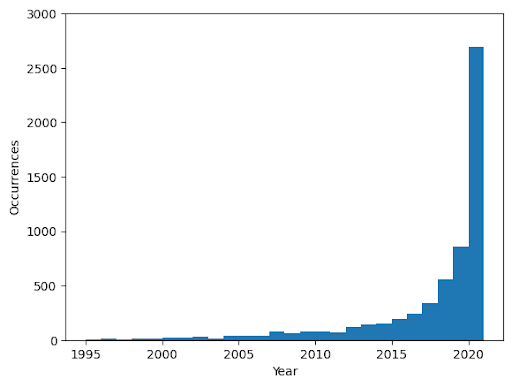
\includegraphics[scale=0.3] {papers_by_year.png}}
    \caption{Growth of Papers Published in ML Hardware over Time.}
    \label{fig}
\end{figure}

After applying these changes, we define a t-SNE visualization on the dataset, 
as pictured in Figure 3. The plot helps to establish underlying patterns and 
relationships in the dataset on a 2-D plane for reader understandability. 
From this plot, we see that there are some strong clusters of papers and 
some much weaker, though still characteristic. \par

Then, after finding the edge list of the dataset, we can plot the degree distribution 
chart of the network, plotting the number of times a paper was cited against the 
frequency of that number of citations, shown in Figure 5 below. \par

\begin{figure}[htbp]
    \centerline{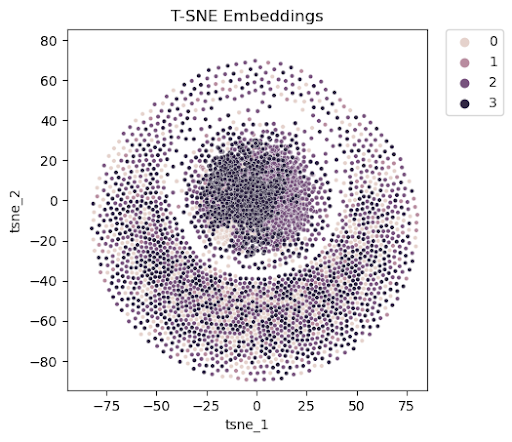
\includegraphics[scale=0.3] {tsne_embeddings.png}}
    \caption{t-SNE Plot of the WoS Dataset.}
    \label{fig}
\end{figure}

From this plot, we establish that the WoS citation network shows 
characteristics of a small-world network, with few nodes exhibiting 
a high number of citations and most having very few citations. 
This result makes sense, as few papers are likely to have a high 
impact, and those that do are likely to influence many papers. \par

\begin{figure}[htbp]
    \centerline{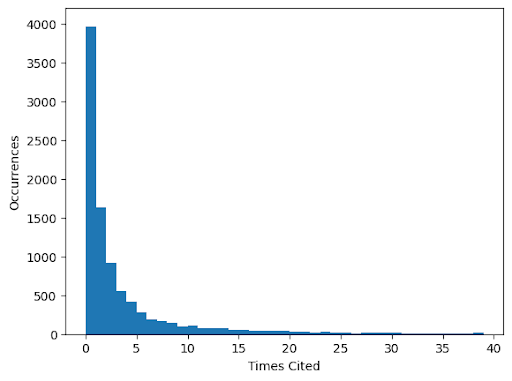
\includegraphics[scale=0.3] {times_cited.png}}
    \caption{Occurrences for papers with certain times cited.}
    \label{fig}
\end{figure}

Looking at the most-cited nodes, we find impactful key publications 
in their respective fields. One such publication is “Equivalent-accuracy 
accelerated neural-network training using analogue memory”, published in 2016 [7]. 
In “Nanoscale memristor device as synapse in neuromorphic systems'' published 
in 2018,  Jo et al. experimentally show a nanoscale memristor working within 
the context of neuromorphic computing \cite{Jo}. In another example, “Memory devices 
and applications for in-memory computing” gives an overview of potential solutions 
to in-memory computing, including solutions closely related to machine learning and 
digital signal processing \cite{Sebastian}. \par

In finding additional outliers, we were also able to distinguish the age of our papers. 
The dataset consisted of papers from the years of 1971 to 2023. The oldest paper, 
the only paper from 1971, was titled “Unit Spike Activity in Coelenteran Neural Network”, 
a paper about temperature spikes in primitive neural nerve networks \cite{Rm}.  \par

While both Cora and Citeseer categorize publications and have vocab dictionaries, 
there are no such categories or dictionaries for Web of Science results. 
Therefore, we utilized the search function to specify the categories to be 
both used and excluded in each search. To match the vocabularies of Cora and 
Citeseer, we utilized spacy for trained keyword extraction models, finding 
the top 10 unigrams with the most significance in each abstract, and used 
these words to construct our vocabulary vectors \cite{keywordspacy}. \par

\begin{figure}[htbp]
    \centering
    \caption{Number of Papers per Year by Category}
    % \captionsetup{labelformat=empty}
    \parbox[b]{.5\linewidth}{
    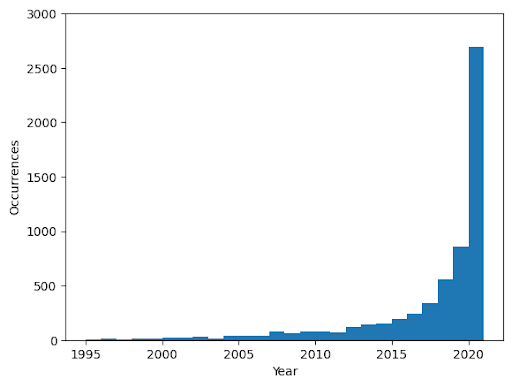
\includegraphics[scale=0.23]{papers_by_year.png}
    \caption{A cat}\label{cat}}
    \parbox[b]{.45\linewidth}{
    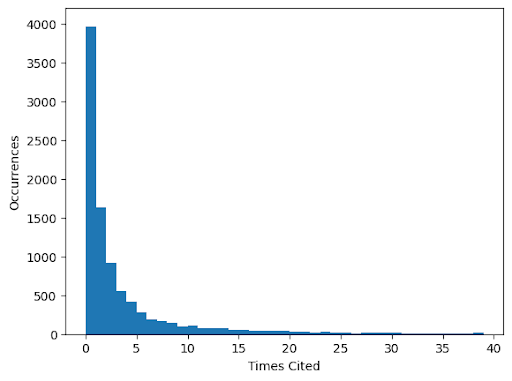
\includegraphics[scale=0.23]{times_cited.png}
    \caption{An elephant}\label{elephant}}
    \hfill
    \parbox[b]{.5\linewidth}{
    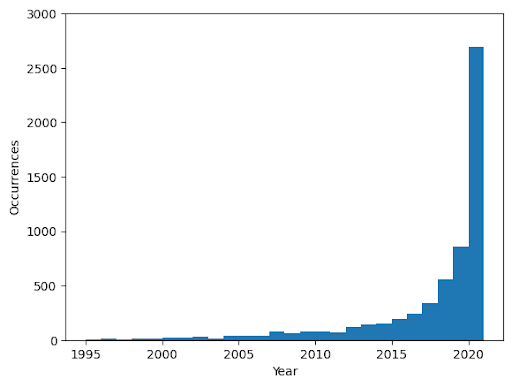
\includegraphics[scale=0.23]{papers_by_year.png}
    \caption{A cat}\label{cat}}
    \parbox[b]{.45\linewidth}{
    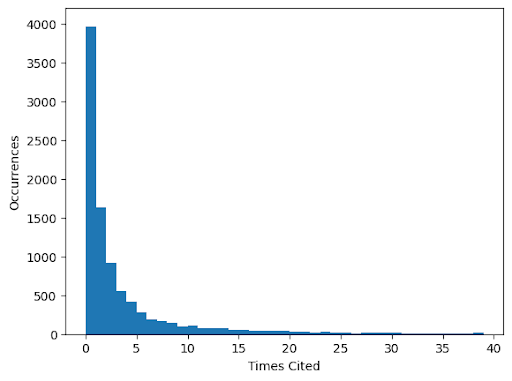
\includegraphics[scale=0.23]{times_cited.png}
    \caption{An elephant}\label{elephant}}
    % \captionsetup{labelformat=simple}
\end{figure}

Next, we examine the structure of each community by computing the mixed edge 
probability, i.e. how many out of the total edges in the graph contain an edge 
from one community to other communities. The mixed edge theoretical probability 
of a certain category, say A, is the probability that any node is in A out of 
all nodes, multiplied by the probability that any node is in any other category. 
We use this simple equation: \par

% TODO: fix new line problem!
\begin{equation}
    Theoretical\; Mixed\; Edge\; Probability(category\; A)
\end{equation}
\begin{equation}
    = (P(node\; in\;A)) (1 - P(node\;in\;A))\label{eq1}
\end{equation}

This number indicates the portion out of all edges that should contain an edge stretching 
from a node in A to a node outside of A if the graph picked edges at random. \par

Our actual mixed edge probability is calculated by: \par
\begin{equation}
    \dfrac{Number\; of\; in\; or\; out\; edges\; of\; a\; community}{Number\; of\; total\; edges}
    \label{eq2}
\end{equation}

As seen in Table 2 below, our actual mixed edge probability is far 
below the theoretical probability in a random graph. \par

% Todo: fix new line problem!
\begin{table}[htbp]
    \caption{Mixed Edge Categorical Analysis}
    \begin{center}
        \begin{tabular}{|c|cccc|}
        \hline
        \textbf{Categories} & \textbf{\textit{Edge}} & \textbf{\textit{ML}} & 
        \textbf{\textit{Neuromorphic}} & \textbf{\textit{Spiking}} \\
        \textbf{} & \textbf{\textit{ML}} & \textbf{\textit{Accelerator}} & 
        \textbf{\textit{Computing}} & \textbf{\textit{NN}} \\
        \hline
        \textbf{\textit{Theoretical}} &\ &\ &\ &\ \\
        \textbf{\textit{Mixed Edge}} &
        0.19813& 0.19256& 0.19051& 0.16663 \\
        \textbf{\textit{Probability}} & \ &\ &\ &\ \\
        \ & \ &\ &\ &\ \\
        \textbf{\textit{Mixed Edge}} & 
        0.02101& 0.06806& 0.09880& 0.05195 \\
        \textbf{\textit{Probability}} & \ &\ &\ &\ \\
        \hline
        \end{tabular}
        \label{tab2}
    \end{center}
\end{table}

% TODO: can be removed later
\ \newline
\ \newline
% \ \newline
% \ \newline
% \ \newline
% \ \newline

There are far fewer edges in between different categories than edges within a category. 
As such, these topics within machine learning are distinct subject areas. \par

\subsection{GNNs}

For our baseline, we used a basic five-layer neural network that is essentially trained on word 
vectors. On Cora, this achieved a 79.43\% accuracy for node classification; 
on Citeseer, this achieved a 71.43\% accuracy. We then implemented a graphical 
convolution network model on the Cora dataset with five feed-forward layers, which 
achieves an accuracy of 71.13\% for link prediction and an accuracy of  86.58\% for 
node classification. For the CiteSeer dataset, we received an accuracy of 74.1
\% on node classification and 84.29\% on link prediction. Similarly, the PubMed dataset 
yielded an accuracy of 78.7\% for both node classification and link prediction. 
These results were further verified through applying a GNN model from DGL, which received 
similar results to the previously mentioned models. This makes sense since Cora is a dataset 
of machine learning papers while CiteSeer has software engineering papers, which is a larger 
domain. Thus, citations are easier to predict in Citeseer. Furthermore, since Citeseer 
has as many keywords as they do papers, and there are half as many keywords in Cora, 
it is more likely that testing on Cora is done on keywords that the model has seen 
before and is thus more accurate. \par

In this regard, these datasets helped to establish a baseline for the expected performance 
of a GNN on the dataset created from the Web of Science after PCA. Following similar methods as 
before, the GNN model for node classification produced an accuracy of 78.06\%, 
while Link prediction fared much better with an accuracy of 82.56\%. 
These results are summarized in Table 3 below. \par 

\begin{table}[htbp]
    \caption{GNN Performance Across Datasets}
    \begin{center}
        \begin{tabular}{|c|cccccc|}
        \hline
        \textbf{Dataset} & \textbf{\textit{Cora}} & \textbf{\textit{CS$^{\mathrm{a}}$}} & \textbf{\textit{PM$^{\mathrm{b}}$}} &
        \textbf{\textit{WoS1$^{\mathrm{c}}$}} & \textbf{WoS2$^{\mathrm{d}}$} & \textbf{WoS3$^{\mathrm{e}}$} \\
        \hline
        \textbf{\textit{Node}} &\ &\ &\ &\ &\ &\ \\
        \textbf{\textit{Classif-}} &
        86.58\%& 74.1\%& 78.7\%& 72.3\%& 76.96\%& 78.06\% \\
        \textbf{\textit{ication}} &\ &\ &\ &\ &\ &\ \\
        
        \ &\ &\ &\ &\ &\ &\ \\

        \textbf{\textit{Link}} &\ &\ &\ &\ &\ &\ \\
        \textbf{\textit{Predic-}} &
        71.13\%& 84.29\%& 78.74\%& 80.8\%& 81.77\%& 82.56\% \\
        \textbf{\textit{tion}} &\ &\ &\ &\ &\ &\ \\

        \hline
        \end{tabular}
        \label{tab1}
        {$^{\mathrm{a}}$CiteSeer.}
        {$^{\mathrm{b}}$PubMed.}
        {$^{\mathrm{c}}$Small WoS.}
        {$^{\mathrm{d}}$Large WoS.}
        {$^{\mathrm{e}}$Large WoS w/ PCA.}
    \end{center}
\end{table}

From the results in the table, we see that our dataset performs weaker than 
PubMed and Cora in terms of node classification and weaker than CiteSeer in 
terms of link prediction. Despite this, our model has the strongest performance 
averaged between node classification and link prediction, even before PCA. It is 
also interesting to note that the larger networks in terms of nodes have a smaller 
difference between the performance of node classification and link prediction, 
WoS by just a few percentage points and PubMed by less than a tenth of a percent. 
Similarly, CiteSeer has the lowest average degree and also performs the 
best for link prediction. \par 

However, one of the strongest limitations in the results of the applied models 
is the lack of knowledge of the cause of performance. The performance of the 
models could be motivated by differences in the structure of the networks due 
to the nature of the associated fields, differences in the databases used to 
curate the networks, and differences in the characteristics of the networks 
themselves. For example, CiteSeer has multiple self-loops, while the other 
networks have few if any. Similarly, Cora and CiteSeer are unconnected, while 
PubMed is connected. Future research on this paper could extend this study to 
homogenize the datasets by removing self-loops, making all graphs connected, 
and applying PCA to all datasets to observe any changes in performance. \par 

Similarly, a limitation in our approach exists in our dataset in the class 
imbalance of the ML Accelerator class having far fewer papers than the other 
classes. This limitation can influence the results of the dataset, such as 
creating a tendency to not classify a node as ML Accelerator since it is 
less likely for a paper to belong to this class. This issue can be addressed 
through solutions such as minority oversampling, creating artificial samples 
of the ML Accelerator class, or majority undersampling, omitting some samples 
of the remaining classes to simulate more balanced classes. However, to 
preserve any information about the underlying structure of the field of 
ML hardware, we assume that this imbalance of classes is a property of 
the field of ML hardware, avoiding any manipulation of the original 
set of samples. \par

For future plans, the most straightforward path is exploring the use of the 
dataset as an academic tool. Cora and CiteSeer are both extensively used as a 
tool for the exploration of machine learning, aiming for the strongest results 
of classification for the dataset. A similar approach can be used for the new 
WoS dataset, observing the results of these high-performing methods in Cora 
or CiteSeer on the WoS dataset. Similarly, this dataset can be used to explore 
new models for classifying or predicting citation networks. Since this dataset 
has different characteristics than all of the others, it may offer insight 
into using new or different models than before. \par

Additionally, the models trained on the WoS dataset can be used for node 
classification or link prediction in a practical sense. By classifying 
papers in the field of machine learning hardware, the model can help 
differentiate papers of the two categories in real life. This also 
applies to link prediction - predicting links on an unpublished paper or 
abstract can provide insight into potential inspiration from other academic 
works. Similar applications of link prediction can assist in finding not only 
papers for inspiration, but also other authors to collaborate with if, 
for example, both authors have similar published papers. \par

\section{Conclusion and Future Work}

Overall, we reached our goals for this project of developing a new dataset 
for papers relating to machine learning hardware for a better understanding 
of the relationships between publications and authors. Through creating a 
dataset that is well explained through node classification and link prediction, 
these results can be reproduced for alternative applications like publication 
classification or potential author collaboration. \par 

In the development of this project, we have had the opportunity to witness 
the application of GNNs on citation networks, in addition to a new dataset. 
So, we have learned of various qualities of citation networks such as their 
degree distribution, clustering coefficient, and their underlying network 
structure, witnessing underlying paper data distribution. We also explore 
GNN model differences between node classification and link prediction. 
Creating a new dataset, we saw that GNNs are effective for node classification 
and link prediction on a new network of machine learning hardware papers. \par

Thus far, we created a dataset of machine learning hardware papers across 
different demographics with classifications to be used in node classification 
and link prediction, quantified in terms of characteristics like degree and 
clustering coefficient, comparing the datasets in terms of traits and GNN performance. 
While the creation of a competing academic dataset is a strong start to our goal, 
our created graph still has opportunities for improvement. \par

\begin{thebibliography}{00}
\bibitem{CoraAccuracy} "Node Classification on Cora", url: https://paperswithcode.com/sota/node-classification-on-cora.
\bibitem{Ucar} T. Ucar, "NESS: Node Embeddings from Static SubGraphs", in arXiv, 2023, url: https://doi.org/10.48550/arXiv.2303.08958. 
\bibitem{Pubmed} National Library of Medicine, "Pubmed", url: https://relational.fit.cvut.cz/dataset/PubMed\_Diabetes.
\bibitem{WoS} Clarivate, "Web of Science", 2023, url: https://www.webofscience.com/wos/woscc/basic-search.
\bibitem{Wade} A. D. Wade, "The semantic scholar academic graph (s2ag)", in Companion Proceedings of the Web Conference 2022, 2022, pp. 739-739.
\bibitem{Sinha} A. Sinha et al., "An overview of microsoft academic service (mas) and applications", in Proceedings of the 24th international conference on world wide web, 2015, pp. 243-246.
\bibitem{Ambrogio} S. Ambrogio et al., "Equivalent-accuracy accelerated neural-network training using analogue memory", Nature, vol. 558, no. 7708, pp. 60-67, 2018.
\bibitem{Jo} Jo SH, Chang T, Ebong I, Bhadviya BB, Mazumder P, Lu W. "Nanoscale memristor device as synapse in neuromorphic systems," in Nano Lett., 10(4):1297-301, 2010, doi: 10.1021/nl904092h.
\bibitem{Sebastian} A. Sebastian, M. Le Gallo, R. Khaddam-Aljameh, and E. Eleftheriou, "Memory devices and applications for in-memory computing", Nature nanotechnology, vol. 15, no. 7, pp. 529-544, 2020.
\bibitem{Rm} B. Rm, "Unit Spike Activity in Coelenteran Neural Network", NATURWISSENSCHAFTEN, vol. 58, no. 3. Springer Verlag 175 Fifth Ave., New York, NY 10010, p. 153, 1971.
\bibitem{keywordspacy} Honnibal, M. \& Montani, I., keyword-spaCy, Natural language understanding with Bloom embeddings, convolutional neural networks and incremental parsing, 2017, url: https://github.com/wjbmattingly/keyword-spacy.
\end{thebibliography}
\end{document}
